%%%%%%%%%%%%%%%%%%%%%%%%%%%%%%%%%%%%%%%%%%%%%%%%%%%%%%%%%%%%%%%%%%%%%%%%%%%%%%%%%
% Document template TEX-STD-A4 by g0hl1n
%
% This document is derived from the TEX-STD-A4 template.
% The TEX-STD-A4 template was released into the public domain.
% For more information, please refer to <http://unlicense.org/>
%   Template-Source:  https://github.com/g0hl1n/LaTeX
%   Template-Author:  Richard 'g0hl1n' Leitner <me@g0hl1n.net>
%   Template-Version: 1.1
%%%%%%%%%%%%%%%%%%%%%%%%%%%%%%%%%%%%%%%%%%%%%%%%%%%%%%%%%%%%%%%%%%%%%%%%%%%%%%%%%
\documentclass[a4paper,12pt]{article} % An article on a4paper with 12pt fontsize
\usepackage[utf8]{inputenc} % input is utf8
\usepackage[ngerman]{babel} % comment-in for new-german, out for english

%----------------------------------------------------------------------------------------
%	META DATA
%----------------------------------------------------------------------------------------
\def \theauthor  {Daniela Pointinger\\Michael Haslauer\\Stefan Winkler\\Johannes Briewasser}
\def \footerauthor {PoiD HasM WinS BriJ}
\def \thedate    {\today}
\def \thetitle   {Softwareentwicklung\\Architektur}
\def \subtitle   {vom 10. Mai 2014}
\def \shorttitle {SWE Architektur}
\def \company    {Fachhochschule Salzburg}
\def \department {itsb-m2013}
\def \version    {1.0}

\author{\theauthor\\\company}
\date{\thedate}
\title{\thetitle}

%----------------------------------------------------------------------------------------
%	PACKAGES
%----------------------------------------------------------------------------------------
\usepackage{geometry} % for page dimensions
\usepackage{fancyhdr} % for custom (fancy) headers and footers
\usepackage{lastpage} % for pagecount
\usepackage{graphicx} % for embedding graphics
\usepackage{listings} % for source listings
\usepackage{hyperref} % for urls and their appearence
\usepackage{color}    % for colored text
\usepackage{fancyvrb} % for custom verbatims
\usepackage{graphicx} % Required for including pictures
\usepackage{float}    % Allows putting an [H] in \begin{figure} to specify the exact location of the figure
\usepackage{wrapfig}  % Allows in-line images such as the example fish picture
\usepackage{blindtext}% for blind text
\usepackage[table,usenames,dvipsnames]{xcolor} % for own color definitions and tables
\usepackage{colortbl}
%\usepackage{arev}		% the arev font
%\usepackage[T1]{fontenc}
\usepackage{multirow} % for multirowed columns in tables
\usepackage{listings} % sourcecode listings
\usepackage{appendix} % for appendices

%----------------------------------------------------------------------------------------
%	DOCUMENT CONFIGRUATION
%----------------------------------------------------------------------------------------
\geometry{top=25mm,left=25mm,right=20mm,bottom=22mm,headsep=10mm,footskip=12mm}

\linespread{1} % Line spacing
%\setlength\parindent{0pt} % remove all indentation from paragraphs

\graphicspath{{./img/}} % Specifies the directory where pictures are stored

%Hyperlink setup
\hypersetup{
    colorlinks,
    citecolor=black,
    filecolor=black,
    linkcolor=black,
    urlcolor=black
}

% Listing Style
\lstdefinestyle{code}{
	breaklines=true,
	frame=single,
	captionpos=b,
	basicstyle=\ttfamily,
}

% Enable custom header & footer
\pagestyle{fancy}

% set the header height (to avoid warnings)
\setlength{\headheight}{14.5pt}

% define my Header
\renewcommand{\headrulewidth}{0.4pt}
\fancyhead[L]{\company}
\fancyhead[C]{\department}
\fancyhead[R]{\shorttitle}

% define my Footer
\renewcommand{\footrulewidth}{0.4pt}
\fancyfoot[L]{\footerauthor}
\fancyfoot[C]{V\version\ $\mid$ \thedate}
\fancyfoot[R]{Page \thepage\ of \pageref{LastPage}}

% COLORS:
\definecolor{titlepagelinecolor}{HTML}{707070} % grey
%\definecolor{titlepagelinecolor}{HTML}{007A04} % green

% rename title of "Listings"
%\renewcommand{\lstlistlistingname}{List of Listings}

% no pagebreak after title:
\let\endtitlepage\relax

\hyphenation{Authenti-cation}

\begin{document}

%----------------------------------------------------------------------------------------
%	TITLE & TABLE OF CONTENTS
%----------------------------------------------------------------------------------------
\begin{titlepage}
\begin{center}
\Large\company\tiny\\
\textcolor{titlepagelinecolor}{\line(1,0){465}\\[1cm]}
\huge
\textbf{\thetitle}\\
\Large \subtitle\\[1cm]
\end{center}
\large
\theauthor\ $\mid$ \department\hfill Version \version\ $\mid$ \thedate\\[1cm]
\textcolor{titlepagelinecolor}{\line(1,0){465}\\[1cm]}
\end{titlepage}

\tableofcontents % Include a table of contents

\newpage
%\setcounter{page}{1} % Reset Page counter


%----------------------------------------------------------------------------------------
%	INHALT
%----------------------------------------------------------------------------------------
\section{Einführung}
Das folgende Dokument beschreibt die Softwarearchitektur des Softwareentwicklungsprojekts "Bahn Zahlsystem". Da es sich hierbei um eine Online-Applikation handelt die über unterschiedliche Wege erreicht werden soll muss ein hierfür geeignetes Architekturkonzept gewählt werden.

\section{Architekturkontept}
Das Projekt \glqq{}Bahn Zahlsystem\grqq{} ist eine Online-Applikation die mehrere Möglichkeiten der Nutzung bietet. Außerdem müssen externe Drittapplikationen in die Applikation integriert werden können. Das Grundkonzept das hier verwendet werden soll ist die Schichtenarchitektur. Diese bietet den Vorteil, dass Änderungen in bestimmten Bereichen nicht die komplette Applikation beeinflussen sondern nur in der jeweiligen Schicht angepasst werden müssen. Außerdem lassen sich in diesem Fall die Komponenten der Schichten auf logischer Ebene trennen und jeder Schicht einen speziellen Aufgabenbereich zuordnen. Die Architektur umfasst dabei die 4 Schichten für:
\begin{itemize}\itemsep2pt
 \item Domänenobjekte und Peristenz
 \item Business-Logik
 \item Benutzeroberfläche
 \item Anbindung Drittsysteme
\end{itemize}
Im folgenden werden die einzelnen Schichten und deren Schnittstellen genauer beschrieben.

\section{Schichtenbeschreibung}
Bei einem Schichtenmodell gilt, dass die einzelnen Layer des Modells nur mit den direkt an einen Layer angrenzende Schichten kommunizieren kann.

\subsection{Domänenobjekte und Persistenz}
In dieser Schicht sind die einzelnen Objekte und deren Metadaten definiert, die für den Einsatz in dieser Domäne nötig sind und in der Applikation verwendet werden. Die Objekte bilden die Schnittstelle zu den konkreten Daten für die Verarbeitung und Durchführung von Prozessen. Der Zugriff von der darüberliegenden Schicht auf Daten erfolgt somit nicht direkt, sondern wird über diese Objekte gekapselt. Sie bietet demnach eine reine Objektschnittstelle. Außerdem befindet sich in dieser Schicht keine weitere Logik, außer derjenigen, die für die Erstellung und Speicherung der Objekte nötig ist.\newline
Eine Bereitstellung der Objekte bzw. der Persistierung von Änderungen in der Datenbank erfolgt nur auf Anfrage. Die darüberliegende Schicht fragt über diese Persistenzschicht an, das Objekt mit den Daten aus der Datenbank zu befüllen. Um geänderte Daten in die Datenbank zu speichern, wird von der darüberliegenden Schicht eine Methode dieser Persistenzschicht aufgerufen.\newline
Die Menge der Domänenobjekte und deren Metadaten ist eine nahezu vollständig definierte Menge. Änderungen in dieser Schicht ergeben weitreichendere Folgen für alle darüber angesiedelten Schichten. Außerdem ist in dieser Schicht die technische Schnittstelle zur Datenbank angesiedelt, sowie die Datenbank selbst.

\subsection{Business-Logik}
Diese Schicht beinhaltet die komplette Logik die für die Abwicklung der Business-Prozesse nötig ist. Sie bildet somit die Use-Cases der Requirement-Engineering Phase ab. Die Logik greift auf die Objekte der unteren Schicht zu und führt Operationen darauf aus. Außerdem erfolgt die komplette Fehlerbehandlung dieser und der darunterliegenden Schichten in dieser Schicht. Lediglich die Benutzeroberfläche beinhaltet ein eigenes Fehlermanagement, da dieses potentiell nicht Teil der selbstentwickelten Lösung sein muss. Die Dienste der Business-Logik stehen den darüberliegenden Schichten als REST-Schnittstelle zur Verfügung die eine Datenschnittstelle via JSON/XML bietet.

\subsection{Benutzeroberfläche}
Die Benutzeroberfläche ist in einer eigenen Schicht gekapselt und ist somit getrennt von der Bunsiness-Logik. Sie beinhaltet alle nötigen Steuerelemente die der Benutzer braucht um Prozesse durchzuführen. Durch die Trennung der Oberfläche können somit Anpassungen vorgenommen werden, ohne das Änderungen in den Schichten darunter nötig sind. Ob es sich bei der Benutzeroberfläche um ein Webinterface oder eine Mobile-App handelt ist damit unerheblich. Außerdem können mehrere unterschiedliche Benutzeroberflächen parallel existieren.

\subsection{Anbindung Drittsysteme}
Die Anbindung von Drittsystemen wird in einer eigenen Schicht gekapselt. Diese Schicht beinhaltet alle nötige Logik um ein Drittsystem nutzen zu können. Die Schnittstellen der Drittsysteme werden somit in einen eigene Schnittstelle umgewandelt die letztendlich von der Business-Logik genutzt werden. Die Business-Logik bekommt somit nichts vom Drittsystem mit, was ein Austauschen leichter möglich macht, sofern die Schnittstelle unverändert bleibt. Die Besonderheit dieser Schicht liegt darin, dass sie sich parallel zur Business-Logik schicht befindet und nicht darunter bzw. darüber. Sie kann somit ebenfalls die Domänenobjekte nutzen, allerdings werden ihre Dienste nur von der Business Logik genutzt und über eine Funktionsschnittstelle bereitgestellt.

\subsection{Schichtendiagramm}
In Abbildung \ref{fig:architektur} ist das Schema der einzelnen Schichten in der Architektur visualisiert.
\begin{figure}[H]
	\centering
	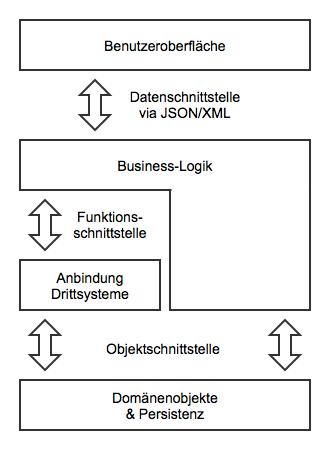
\includegraphics[width=0.5\textwidth]{img/architektur.png}
	\caption{Schema der Schichten}
	\label{fig:architektur}
\end{figure}
Zu erkennen sind außerdem die einzelnen Schnittstellen und um welchen Typ von Schnittstelle es sich hierbei handelt.

\newpage
%----------------------------------------------------------------------------------------
%	LISTS
%----------------------------------------------------------------------------------------
% List of Figures
\newpage
\phantomsection
\addcontentsline{toc}{section}{\listfigurename}
\listoffigures

% List of Tables
%\newpage
%\phantomsection
%\addcontentsline{toc}{section}{\listtablename}
%\listoftables

% List of Listings
%\newpage
%\phantomsection
%\addcontentsline{toc}{section}{\lstlistlistingname}
%\lstlistoflistings

% Bibliography
%\newpage
%\phantomsection
%\addcontentsline{toc}{section}{Literatur}
%\bibliographystyle{plain}
%\bibliography{bibliography}


%----------------------------------------------------------------------------------------
%	APPENDICES
%----------------------------------------------------------------------------------------
\begin{appendix}
%\section{Geräte-Konfigurationen}
%\label{apx:configs}
%\subsection{Router1}
%\label{apx:router_conf:1}
%\lstinputlisting[style=code,caption={Konfiguration Router1}]{configs/config_R1_01.txt}
%
%\subsection{Router2}
%\label{apx:router_conf:2}
%\lstinputlisting[style=code,caption={Konfiguration Router2}]{configs/config_R2_01.txt}
%
%\subsection{Router3}
%\label{apx:router_conf:3}
%\lstinputlisting[style=code,caption={Konfiguration Router3}]{configs/config_R3_01.txt}
%
%\subsection{ASA}
%\label{apx:router_conf:asa}
%\lstinputlisting[style=code,caption={Konfiguration ASA}]{configs/config_ASA_01_vor_VPN.txt}

\end{appendix}



%----------------------------------------------------------------------------------------

\end{document}
